% figures/fig2_access_retention.tex
\begin{figure}[t]
  \centering
  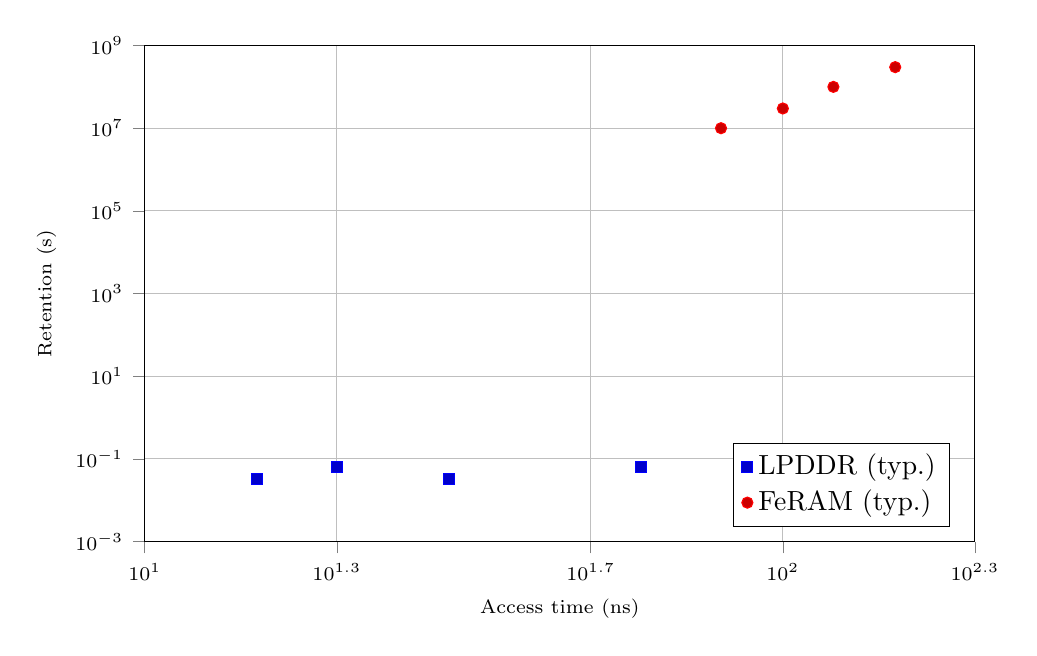
\begin{tikzpicture}
    \begin{loglogaxis}[
      width=\columnwidth,
      height=0.65\columnwidth,
      xlabel={Access time (ns)},
      ylabel={Retention (s)},
      legend style={at={(0.97,0.03)},anchor=south east},
      legend cell align=left,
      grid=both,
      tick align=outside,
      tickpos=left,
      xmin=10, xmax=200,
      ymin=1e-3, ymax=1e9,
      xtick={10,20,50,100,200},
      ytick={1e-3,1e-1,1e1,1e3,1e5,1e7,1e9},
      clip=false,
      label style={font=\scriptsize},
      tick label style={font=\scriptsize}
    ]

    % LPDDR
    \addplot+[only marks, mark=square*, mark size=2pt]
    coordinates {
      (15, 3.2e-2)
      (20, 6.4e-2)
      (30, 3.2e-2)
      (60, 6.4e-2)
      (100, 3.2e-2)
    };
    \addlegendentry{LPDDR (typ.)}

    % FeRAM
    \addplot+[only marks, mark=*, mark size=2pt]
    coordinates {
      (80, 1.0e7)
      (100, 3.0e7)
      (120, 1.0e8)
      (150, 3.0e8)
    };
    \addlegendentry{FeRAM (typ.)}

    \end{loglogaxis}
  \end{tikzpicture}
  \vspace{-0.6em}
  \caption{Access time vs. retention. LPDDR delivers short access with volatile retention; FeRAM offers longer retention with moderate access.}
  \label{fig:access_retention_lpddr_feram}
\end{figure}
